%!Tex Program = xelatex
%------------------------------------------------------------------------------%
% Compile this document, by following instructures below:
% > xelatex assignment.tex
% > xelatex assignment.tex
%------------------------------------------------------------------------------%
\documentclass[no-math, compress]{beamer}
%------------------------------------------------------------------------------%
% Add "handout" flag to export a handout version
% \documentclass[no-math, handout, compress]{beamer}
%------------------------------------------------------------------------------%

\mode<presentation>

% beamer 导言区设置
% beamer 设置区
\usepackage[UTF8, noindent]{ctexcap}
\usepackage{graphicx}
\usetheme{CambridgeUS}


%---------------------------------拯救下标环境---------------------------------%
\makeatletter
% save the meaning of \@footnotetext
\let\BEAMER@footnotetext\@footnotetext
\makeatother
%------------------------------------------------------------------------------%


%----------------------------------必要库支持----------------------------------%
\usepackage{xcolor}
\usepackage{tikz}
\usepackage{clrscode}
\usepackage{animate}
%------------------------------------------------------------------------------%


%--------------------------------添加书签超链接--------------------------------%
% \usepackage[unicode=true,colorlinks=false,pdfborder={0 0 0}]{hyperref}
% 在此处修改打开文件操作
\hypersetup{
    bookmarks=true,         % show bookmarks bar?
    pdftoolbar=true,        % show Acrobat’s toolbar?
    pdfmenubar=true,        % show Acrobat’s menu?
    pdffitwindow=true,      % window fit to page when opened
    pdfstartview={FitV},    % fits the width of the page to the window
    pdfnewwindow=true,      % links in new PDF window
}
% 在此处添加文章基础信息
\hypersetup{
    pdftitle={},
    pdfauthor={polossk},
    pdfsubject={},
    pdfcreator={XeLaTeX},
    pdfproducer={XeLaTeX},
    pdfkeywords={},
}
%------------------------------------------------------------------------------%


%---------------------------------设置字体大小---------------------------------%
\usepackage{type1cm}
% 字号与行距,统一前缀s(a.k.a size)
\newcommand{\sChuhao}{\fontsize{42pt}{63pt}\selectfont}                 % 初号, 1.5倍
\newcommand{\sYihao}{\fontsize{26pt}{36pt}\selectfont}                  % 一号, 1.4倍
\newcommand{\sErhao}{\fontsize{22pt}{28pt}\selectfont}                  % 二号, 1.25倍
\newcommand{\sXiaoer}{\fontsize{18pt}{18pt}\selectfont}                 % 小二, 单倍
\newcommand{\sSanhao}{\fontsize{16pt}{24pt}\selectfont}                 % 三号, 1.5倍
\newcommand{\sXiaosan}{\fontsize{15pt}{22pt}\selectfont}                % 小三, 1.5倍
\newcommand{\sSihao}{\fontsize{14pt}{21pt}\selectfont}                  % 四号, 1.5倍
\newcommand{\sHalfXiaosi}{\fontsize{12.5pt}{16.25pt}\selectfont}        % 半小四, 1.25倍
\newcommand{\sLargeHalfXiaosi}{\fontsize{13pt}{19pt}\selectfont}        % 半小四, 1.5倍
\newcommand{\sXiaosi}{\fontsize{12pt}{14.4pt}\selectfont}               % 小四, 1.25倍
\newcommand{\sLargeWuhao}{\fontsize{11pt}{11pt}\selectfont}             % 大五, 单倍
\newcommand{\sWuhao}{\fontsize{10.5pt}{10.5pt}\selectfont}              % 五号, 单倍
\newcommand{\sXiaowu}{\fontsize{9pt}{9pt}\selectfont}                   % 小五, 单倍
%------------------------------------------------------------------------------%


%---------------------------------设置中文字体---------------------------------%
\usepackage{fontspec}
% 使用 Adobe 字体
\newcommand\adobeSog{Adobe Song Std}
\newcommand\adobeHei{Adobe Heiti Std}
\newcommand\adobeKai{Adobe Kaiti Std}
\newcommand\adobeFag{Adobe Fangsong Std}
\newcommand\codeFont{Consolas}
% 设置字体
\defaultfontfeatures{Mapping=tex-text}
\setCJKmainfont[ItalicFont=\adobeKai, BoldFont=\adobeHei]{\adobeSog}
\setCJKsansfont[ItalicFont=\adobeKai, BoldFont=\adobeHei]{\adobeSog}
\setCJKmonofont{\codeFont}
\setmonofont{\codeFont}
% 设置字体族
\setCJKfamilyfont{song}{\adobeSog}      % 宋体
\setCJKfamilyfont{hei}{\adobeHei}       % 黑体
\setCJKfamilyfont{kai}{\adobeKai}       % 楷体
\setCJKfamilyfont{fang}{\adobeFag}      % 仿宋体
% 用于页眉学校名,特殊字体,powerby https://github.com/ecomfe/fonteditor
\setCJKfamilyfont{nwpu}{nwpuname}
% 新建字体命令,统一前缀f(a.k.a font)
\newcommand{\fSong}{\CJKfamily{song}}
\newcommand{\fHei}{\CJKfamily{hei}}
\newcommand{\fFang}{\CJKfamily{fang}}
\newcommand{\fKai}{\CJKfamily{kai}}
\newcommand{\fNWPU}{\CJKfamily{nwpu}}
%------------------------------------------------------------------------------%


%------------------------------添加插图与表格控制------------------------------%
\usepackage{graphicx}
\usepackage[font=small,labelsep=quad]{caption}
\usepackage{wrapfig}
\usepackage{multirow,makecell}
\usepackage{longtable}
\usepackage{booktabs}
\usepackage{tabularx}
\usepackage{setspace}
\captionsetup[table]{labelfont=bf,textfont=bf}
% 修复标题格式设置
\makeatletter
\let\@@magyar@captionfix\relax
\makeatother
%------------------------------------------------------------------------------%


%---------------------------------拯救下标环境---------------------------------%
\makeatletter
% restore the meaning of \@footnotetext
\let\@footnotetext\BEAMER@footnotetext
% patch the relevant command to do single spacing in footnotes
\expandafter\patchcmd\csname beamerx@\string\beamer@framefootnotetext\endcsname
{\reset@font}
{\def\baselinestretch{\setspace@singlespace}\reset@font}
{}{}
\makeatother
%------------------------------------------------------------------------------%


%---------------------------------设置引用格式---------------------------------%
\setbeamertemplate{caption}[numbered]
\newcommand\myreference[1]{[\ref{#1}]}
\newcommand\eqrefe[1]{式(\ref{#1})}
% 增加 \ucite 命令使显示的引用为上标形式
\newcommand{\ucite}[1]{$^{\mbox{\scriptsize \cite{#1}}}$}
%------------------------------------------------------------------------------%


%--------------------------------设置定理类环境--------------------------------%
\newtheorem{myexample}{例}
\newtheorem{thm}{定理}
\newtheorem{mythm}{定理}
\newtheorem{myguess}{猜想}
\newtheorem{mydef}{定义}
\newtheorem{mysolve}{解}
\newtheorem{myalgo}{算法}
\renewcommand\proofname{证明}
%------------------------------------------------------------------------------%


%--------------------------设置中文段落缩进与正文版式--------------------------%
\XeTeXlinebreaklocale "zh"       %使用中文的换行风格
\XeTeXlinebreakskip = 0pt plus 1pt    %调整换行逻辑的弹性大小
%------------------------------------------------------------------------------%


%----------------------------------添加代码控制--------------------------------%
\usepackage{listings}
\lstset{
    basicstyle=\footnotesize\ttfamily,
    numbers=left,
    numberstyle=\tiny,
    numbersep=5pt,
    tabsize=4,
    extendedchars=true,
    breaklines=true,
    identifierstyle=\color[HTML]{984ea3}\bfseries,
    keywordstyle=\color[HTML]{377eb8}\bfseries,
    numberstyle=\color[HTML]{e41a1c},
    commentstyle=\color[HTML]{4daf4a}\bfseries,
    stringstyle=\color[HTML]{ff7f00}\ttfamily\bfseries,
    rulesepcolor=\color[HTML]{cccccc},
    showspaces=false,
    showtabs=false,
    frame=shadowbox,
    framexrightmargin=5pt,
    framexbottommargin=4pt,
    showstringspaces=false,
    escapeinside=`', % 逃逸字符(1左面的键),用于显示中文
}
\renewcommand{\lstlistingname}{CODE}
\lstloadlanguages{% Check Dokumentation for further languages, page 12
    Pascal, C++, Java, Ruby, Python, Matlab, R, Haskell, Mathematica
}
%------------------------------------------------------------------------------%


%-----------------------------参考文献脚标格式配置-----------------------------%
\usepackage[backend=bibtex,citestyle=authoryear,sorting=none,doi=false,url=false]{biblatex}
\setbeamertemplate{bibliography item}[text]
\setbeamerfont{footnote}{size = \tiny}
%------------------------------------------------------------------------------%


\endinput

% 这是简单的beamer的导言区设置,不能单独编译。

% plugins
\usepackage{math-symbols}

% emph
\newcommand\blueText[1]{\textcolor{blue}{\bf #1}}
\newcommand\greenText[1]{\textcolor{green}{\bf #1}}
\newcommand\redText[1]{\textcolor{red}{\bf #1}}
\newcommand\violetText[1]{\textcolor{violet}{\bf #1}}

% 指定相关数据文件路径
\graphicspath{{images/}{animations/}} % 图片与动画文件
\addbibresource{reference.bib} % BibTeX 数据文件及位置

\begin{document}

% 添加所有代码片段
\defverbatim[colored]\codeTipHelloWorld{
\begin{lstlisting}[
	language={C++},
	emph = {std},
	emphstyle = {\color{green}}
]
#include <iostream>
using namespace std;

int main()
{
    cout << "Hello World!" << endl;
    return 0;
}
\end{lstlisting}
}


\defverbatim[colored]\codeTipHaskell{
\begin{lstlisting}[
	language={Haskell}
]
qsort :: (Ord a) => [a] -> [a]
qsort [] = []
qsort (x:xs) =
    let leq = [a | a <- xs, a <= x]
        gt = [a | a <- xs, a > x]
        in qsort leq ++ [x] ++ qsort gt
\end{lstlisting}
}

\endinput
% 这是所用到的代码片段,不能单独编译。


\title{主标题}
\subtitle{副标题}
\institute{单位名称}
\author{报告人}
\date{\today}
\subject{}
\keywords{}

\begin{frame}
    \titlepage
    {\tiny 其他应当在首页出现的内容}
\end{frame}


\begin{frame}{报告内容}
    \tableofcontents
\end{frame}


\section{列表环境}


\begin{frame}{列表环境}{依次高亮的列表}
    \begin{itemize}[<+-| alert@+>]
        \item 内容测试~依次高亮的列表
        \item 内容测试~依次高亮的列表
        \item 内容测试~依次高亮的列表
        \item 内容测试~依次高亮的列表
    \end{itemize}
\end{frame}


\begin{frame}{列表环境}{普通列表}
    \begin{itemize}
        \item 内容测试~普通列表
        \item 内容测试~普通列表
        \item 内容测试~普通列表
        \item 内容测试~普通列表
    \end{itemize}
\end{frame}


\section{图片环境}


\begin{frame}{图片环境}{插入图片}
    \begin{center}
        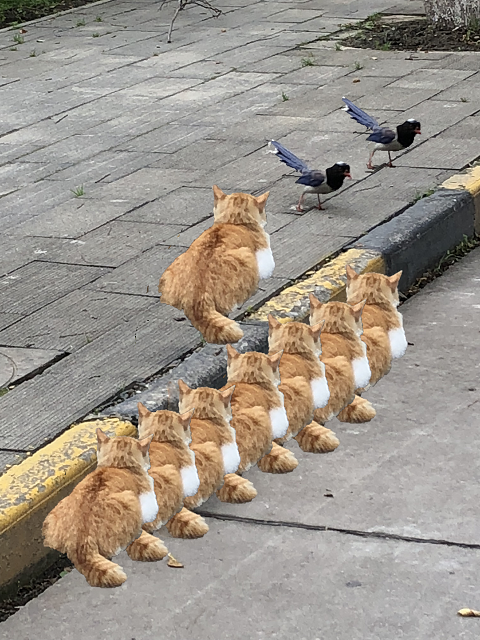
\includegraphics[height=0.6\textheight]{image01}
    \end{center}
\end{frame}


\begin{frame}{图片环境}{插入图片并且添加标题}
    \begin{figure}
        \centering
        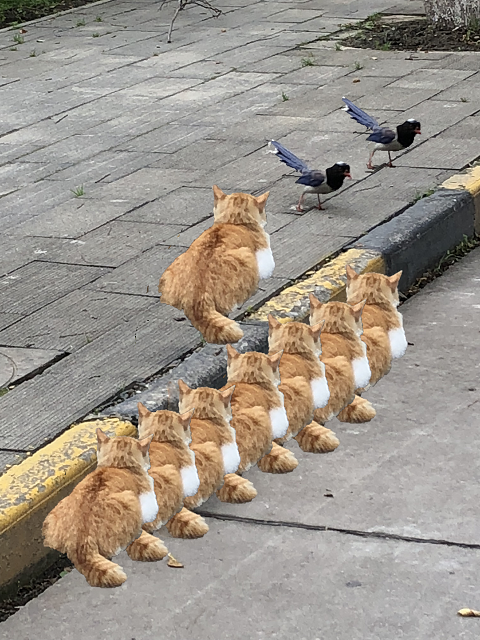
\includegraphics[height=0.6\textheight]{image01}
        \caption{测试插图并标题}
    \end{figure}
\end{frame}


\begin{frame}{图片环境}{插入图片并且添加描述}
    \begin{figure}
        \centering
        \begin{minipage}[t]{0.4\textwidth}
            \centering
            这里有大段大段的描述描述,省略不写。
            这里有大段大段的描述描述,省略不写。
            这里有大段大段的描述描述,省略不写。
            这里有大段大段的描述描述,省略不写。
        \end{minipage}
        \qquad
        \begin{minipage}[t]{0.4\textwidth}
            \centering\vspace{0pt}
            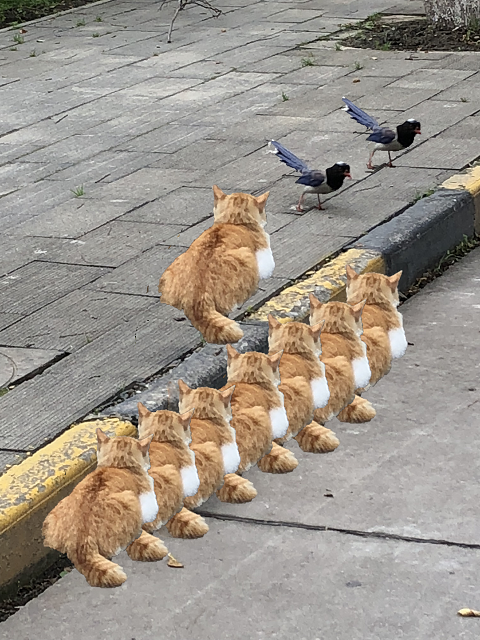
\includegraphics[width=0.8\textwidth]{image01}
        \end{minipage}
        \caption{测试插图并描述}
    \end{figure}
\end{frame}


\begin{frame}{图片环境}{插入图片并且添加描述}
    \begin{figure}
        \centering
        \begin{minipage}[t]{0.4\textwidth}
            \centering\vspace{0pt}
            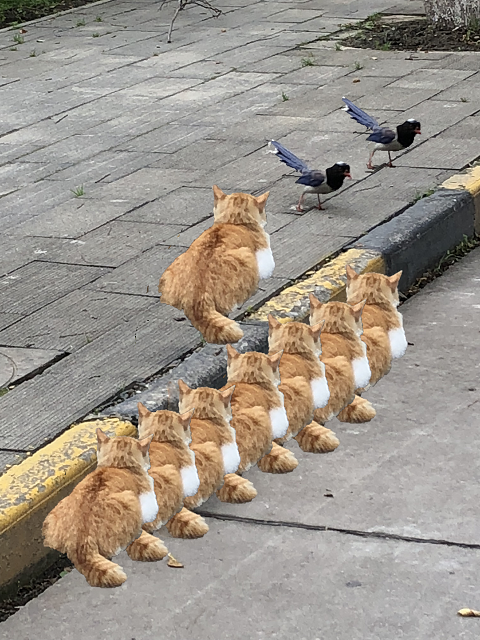
\includegraphics[width=0.8\textwidth]{image01}
        \end{minipage}
        \qquad
        \begin{minipage}[t]{0.4\textwidth}
            \centering
            这里有大段大段的描述描述,省略不写。
            这里有大段大段的描述描述,省略不写。
            这里有大段大段的描述描述,省略不写。
            这里有大段大段的描述描述,省略不写。
        \end{minipage}
        \caption{测试插图并描述}
    \end{figure}
\end{frame}


\begin{frame}{图片环境}{插入两张图片并分别标题}
    \begin{figure}
        \centering
        \begin{minipage}[t]{0.4\textwidth}
            \centering
            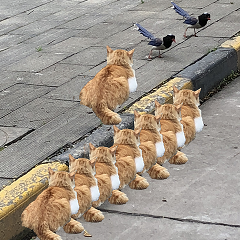
\includegraphics[width=0.8\textwidth]{thumbnail-image01}
            \caption{左图}
        \end{minipage}
        \qquad
        \begin{minipage}[t]{0.4\textwidth}
            \centering
            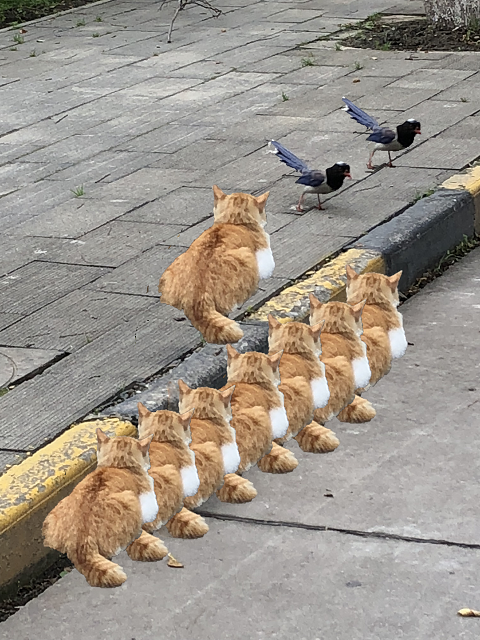
\includegraphics[width=0.8\textwidth]{image01}
            \caption{右图}
        \end{minipage}
        \caption{插入两张图片并分别标题}
    \end{figure}
\end{frame}


\begin{frame}{图片环境}{插入两张图片并按顶部对齐}
    \vspace{-1em}
    \begin{figure}
        \centering
        \begin{minipage}[t]{0.4\textwidth}
            \centering\vspace{0pt}
            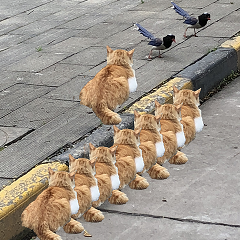
\includegraphics[width=0.8\textwidth]{thumbnail-image01}
            \caption{左图}
        \end{minipage}
        \qquad
        \begin{minipage}[t]{0.4\textwidth}
            \centering\vspace{0pt}
            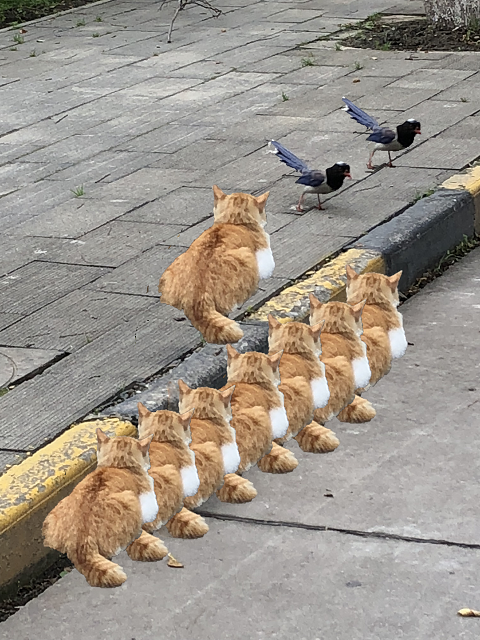
\includegraphics[width=0.8\textwidth]{image01}
            \caption{右图}
        \end{minipage}
        \caption{插入两张图片并按顶部对齐}
    \end{figure}
\end{frame}


\section{参考文献}


\begin{frame}{参考文献}{通过脚注方式引用}
    \begin{itemize}[]
        \item 完全展示\footfullcite{bourdin2000numerical}
        \item 简要展示\footcite{bourdin2000numerical}
        \item 完全展示\footfullcite{MathSymbolsinLaTeXbypolossk}
        \item 简要展示\footcite{MathSymbolsinLaTeXbypolossk}
    \end{itemize}
\end{frame}


\section{其他组件}


\subsection{插入标准三线表}


\begin{frame}{其他组件}{插入标准三线表}
    \begin{table}
        \centering
        \begin{tabular}{ccc}
            \toprule
            Parameters & 5            & 7            \\
            \midrule
            Score A    & 5.188528e-04 & 5.219664e-04 \\
            Score B    & 5.284482e-02 & 4.869455e-02 \\
            \bottomrule
        \end{tabular}
        \caption{标准三线表}
    \end{table}
\end{frame}


\subsection{插入动画}


\begin{frame}{其他组件}{插入动画}
    \begin{center}
        \animategraphics[height=0.5\textheight, autoplay, loop]{10}{animation_wangjz_}{00}{51}
    \end{center}
\end{frame}


\subsection{强调文字}


\begin{frame}{其他组件}{强调文字}
    \begin{itemize}
        \item 内容测试~\blueText{强调文字}环境
        \item 内容测试~\greenText{强调文字}环境
        \item 内容测试~\redText{强调文字}环境
        \item 内容测试~\violetText{强调文字}环境
    \end{itemize}
\end{frame}


\subsection{插入代码}


\begin{frame}[fragile]{其他组件}{插入代码}
    C++ 程序代码 \\
    \begin{center}
        \codeTipHelloWorld
    \end{center}
\end{frame}


\begin{frame}[fragile]{其他组件}{插入代码}
    Haskell 程序代码 \\
    \begin{center}
        \codeTipHaskell
    \end{center}
\end{frame}


\section{Summary}


\begin{frame}
    \begin{center}
        {\Huge \it 谢谢大家!}
    \end{center}
\end{frame}


\end{document}
